\section{24GHz experiments}\label{ghz-experiments}

\subsection{Background}\label{background}

Before going into an account of the the project, let us look at some of
the pros and cons of using this equipment and what is already
known about wireless transmission in the 24 GHz spectrum. We have
already noted that the equipment is affordable. The advertised
throughput of 1.4Gb/s presumably means 700Mb/s in each direction, but
that would provide a satisfactory connection for a hundred or
so residences. Moreover, transmission in this frequency is much
less likely to be affected by tidal reflection (a significant problem
in the Highlands and Islands)

There are some significant drawbacks, though.

\begin{itemize}
\item
  In the UK, the 24.050--24.350GHz band is partitioned into three
  sub-bands\footnote{\href{http://www.ofcom.org.uk/static/archive/ra/publication/ra_info/ra365.htm}{Ofcom
    UK Bandplan}}, and these devices can use two of them. Of these two, one
  is reserved for government and amateur radio use and is not allowed
  for general use and the last is permitted at extremely low power
  densities ($1.5\,\text{mW}/\text{m}^2$ as opposed to the although
  the $13\,\text{W}/\text{m}^2$
  supported by the equipment.  We obtained a ``non-operational''
  licence from Ofcom in order to test the equipment at the advertised
  power and in both sub-bands.
\item
  Several of the links used by Tegola and related projects are longer 
  than 13km
\item
  Transmission in higher frequencies is adversely affected by high 
  humidity and high temperatures. Scotland benefits from only one of 
  these.
\item
  The Ubiquiti equipment uses substantially more power than their 5GHz 
  offerings -- about 40W. This would make it unsuitable for solar and 
  wind-powered relays.
\end{itemize}

Our initial plan was to test the equipment on existing Tegola
relays one is a 6.5km link; the second 15.5km. Although the latter is
over the advertised range, even a substantial fraction of the
advertised throughput would be useful.

The following is a roughly chronological account of the project.
The initial installation was done during a period of very high winds
in early January 2014.

\subsection{Power output calculations}

Expanding on the first bullet point above,
Ofcom has this to say about the part
of the 24GHz radio spectrum used by this equipment in the
UK Bandplan\footnote{\url{http://www.ofcom.org.uk/static/archive/ra/publication/ra_info/ra365.htm}}:

\begin{quotation}
  \itshape
  Non-government low power devices in the radiolocation services are
  limited to:
  
  \vspace{\baselineskip}\noindent
  \begin{enumerate}[(a)]
  \item Portable and fixed applications between 24.15-24.25 GHz; and
  \item Mobile applications between 24.25-24.35 GHz on a NIB to the
    radionavigation service
  \end{enumerate}

  \vspace{\baselineskip}\noindent
  Power flux-density at 10 metres from the system antenna in the\\
  direction of maximum radiation is not to exceed $1.5\,\text{mW}/\text{m}^2$
  without approval

  \vspace{\baselineskip}\noindent
  24.05-24.25 GHz is used by the Amateur service. The part of the
  allocation between 24.05 and 24.150 GHz may only be used with
  written consent of the Secretary of State.

  \vspace{\baselineskip}\noindent
  Home Office/Office of The Scottish Executive for the Emergency
  Services between 24.05-24.15 GHz

  \vspace{\baselineskip}\noindent
  ISM apparatus may use the band 24.0-24.25 GHz.
\end{quotation}

\vspace{\baselineskip}
Also, the UK
Spectrum Strategy 2000 (appendix
B)\footnote{\url{http://www.ofcom.org.uk/static/archive/ra/topirum-strat/future/strat00/appendixb.pdf}}
allows this frequency range to be
used for ``Technology Development'' for low-power fixed and portable
devices. In this context, ``low-power'' means less than
$1.5\,\text{mW}/\text{m}^2$.

The regulations are confusingly laid out, it would appear from
the arrangement of the text that the sentence ``The part of the
allocation between 24.05 and 24.15 GHz may only be used\ldots{}''
pertains only to the amateur service, but it seems to be a global
restriction, particularly since another Ofcom document on
Vehicle Mounted Radar
Detectors\footnote{\url{http://www.ofcom.org.uk/static/archive/ra/topics/research/rtcg/projects/project706.pdf}}
mentions that the police use this part of the
band for radar speed meters.

So generally it is allowed to use this equipment in the UK, it is
just necessary to check the output power and keep away from the bottom
half of the band. The airFibre datasheet\footnote{\url{http://www.ubnt.com/downloads/datasheets/airfiber/airFiber_DS.pdf}}
gives dBm and the
government, gives the permitted radiation energy per unit area at 10
meters from the system. So we need to do a bit of arithmetic.
\begin{figure}
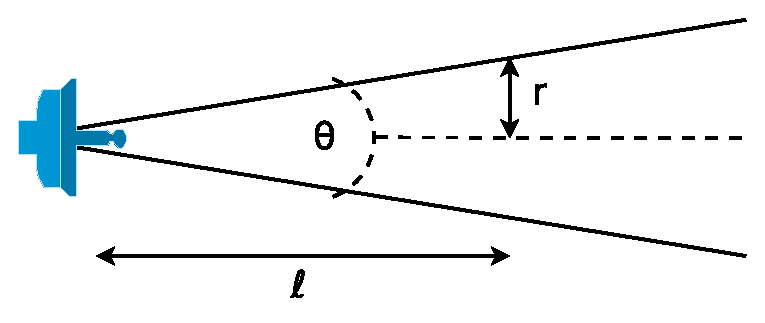
\includegraphics[width=0.5\textwidth]{radiation-cone}
\caption{Directional radiation cone}
\label{fig:cone}
\end{figure}

The datasheet says that the beam-width is less than 3.5$^\circ$. Let's make a
simplifying assumption that it is exactly that width and further that
the cross-section of the main lobe of radiation is circular as
depiceted in figure~\ref{fig:cone}. The radius of the cross-section will be,
\begin{equation}
r = \ell\, \sin\left(\frac{\theta}{2}\right) 
  = 10\,\text{m} \times \sin\left(1.75^\circ\right) = 0.m\,\text{m}
\end{equation}
The area of this circle is, $\pi r^2 = 0.3 \text{m}^2$.

So now, how much power goes through one square meter when
transmitting at 33 dBm?
\begin{equation}
\label{eq:dens2power}
p = \frac{10^{\frac{1}{10}\beta}}{a}  = \frac{10 ^ {\frac{33}{10}\,\text{dBm}}}{0.3\,\text{m}^2} = 
\frac{1995\,\text{mW}}{0.3\,\text{m}^2} = 6.7\,\text{W}/\text{m}^2
\end{equation}
Clearly this is well in excess of the permitted output power.

\subsection{Link budgets}

This experiment is meant to compare the real world performance against
the vendor's claims, but first let us see how the claims stack up
against the theoretical performance. To get an upper bound on possible
throughput we use the Friis Transmission Equation,

\begin{equation}
\label{eq:friis}
  P_r = P_t + G_t + G_r + 20 \log\left(\frac{\lambda}{4\pi d}\right)
\end{equation}
where $P_t$ and $P_r$ are the transmitted and received power levels,
$G_t$ and $G_r$ are the gains of the antennae at either end and the
last term describes the path loss due to distance and wavelength. This
is an ideal model and doesn't account for other real-world sources of
loss.

We will consider two cases, the usual legal limit and the
$33\,\text{dBm}$ transmit power. We know the legal limit is
$1.5\,\text{mW}/\text{m}^2$ so again we need to do some arithmetic
using equation~\ref{eq:dens2power} in the reverse direction,
\begin{equation}
\frac{10^{\frac{1}{10}\beta}}{0.3\,\text{m}^2} = 1.5\,\text{mW}/\text{m}^2
\end{equation}
which we can re-arrange and solve for $P_t + G_t = \beta =
-3.5\,\text{dBm}$.

To make use of equation~\ref{eq:friis} we need some more
information. To find the wavelength, we use,
\begin{equation}
\lambda = \frac{c}{f} = \frac{299,792,458\,\text{m}/\text{s}}{24
  \times 10^9 \,\text{Hz}} = 0.0125\,\text{m}
\end{equation}
where $c$ is the speed of light. We also look up in the datasheet and
see that the receive gain, $G_r$ is $23\,\text{dB}$.

So as a first calculation, let us see what receive power can be
expected at $13\,\text{km}$,
$$
\begin{array}{rcl}
P_r &=& -3.5\,\text{dBm} + 23\,\text{dB} +
20\log\left(\frac{0.0125\,\text{m}}{4\pi \times
  13,000\,\text{m}}\right)\\
    &=& -3.5 + 23 - 142 = -122\,\text{dBm}\\
\end{array}
$$
Referring again to the data sheet, we find that the weakest signal
that can sustain a connection (at about $3\,\text{Mbps}$ since we would
need to use $10\,\text{MHz}$ wide channels -- the datasheet is
misleading on this point since it only quotes throughput numbers for
$50\,\text{MHz}$ wide channels) is
$-95\,\text{dBm}$. At the legal limit we are $27\,\text{dB}$ or about
500 times weaker than we need to be to sustain a link at the
advertised distance. Clearly transmitting at $33\, \text{dBm}$ with
our non-operational licence this is feasible, indeed we have $12\,\text{dB}$
margin to spare which, again referring to the datasheet, should net us
$128\,\text{Mbps}$ over this distance.

So let us ask another question. Over what distance is it possible to
sustain the maximum advertised throughput? For this, according to the
datasheet, we need a receive power of at least $P_r =
-58\,\text{dBm}$. Solving equation~\ref{eq:friis} for the distance,
$d$, we get,
\begin{equation}
d = \frac{\lambda}{4\pi} 10^{\frac{1}{20}\left(-P_r + P_t + G_r + G_t\right)}
\end{equation}
which works out to all of $7.5\,\text{m}$ at the regulatory limit and
$500\,\text{m}$ at $33\,\text{dBm}$.

In our case we are planning to run this on links at most
$6\,\text{km}$ where the same calculations say that we can expect a
receive signal level of around $-79\,\text{dBm}$ which means that
using $40\,\text{MHz}$ wide channels we should be able to solidly
sustain links at $256\,\text{Mbps}$ or better for shorter links.

\subsection{Initial configuration and testing}
\label{december-2013-initial-configuration-and-testing}

\begin{wrapfigure}{r}{0.3\textwidth}
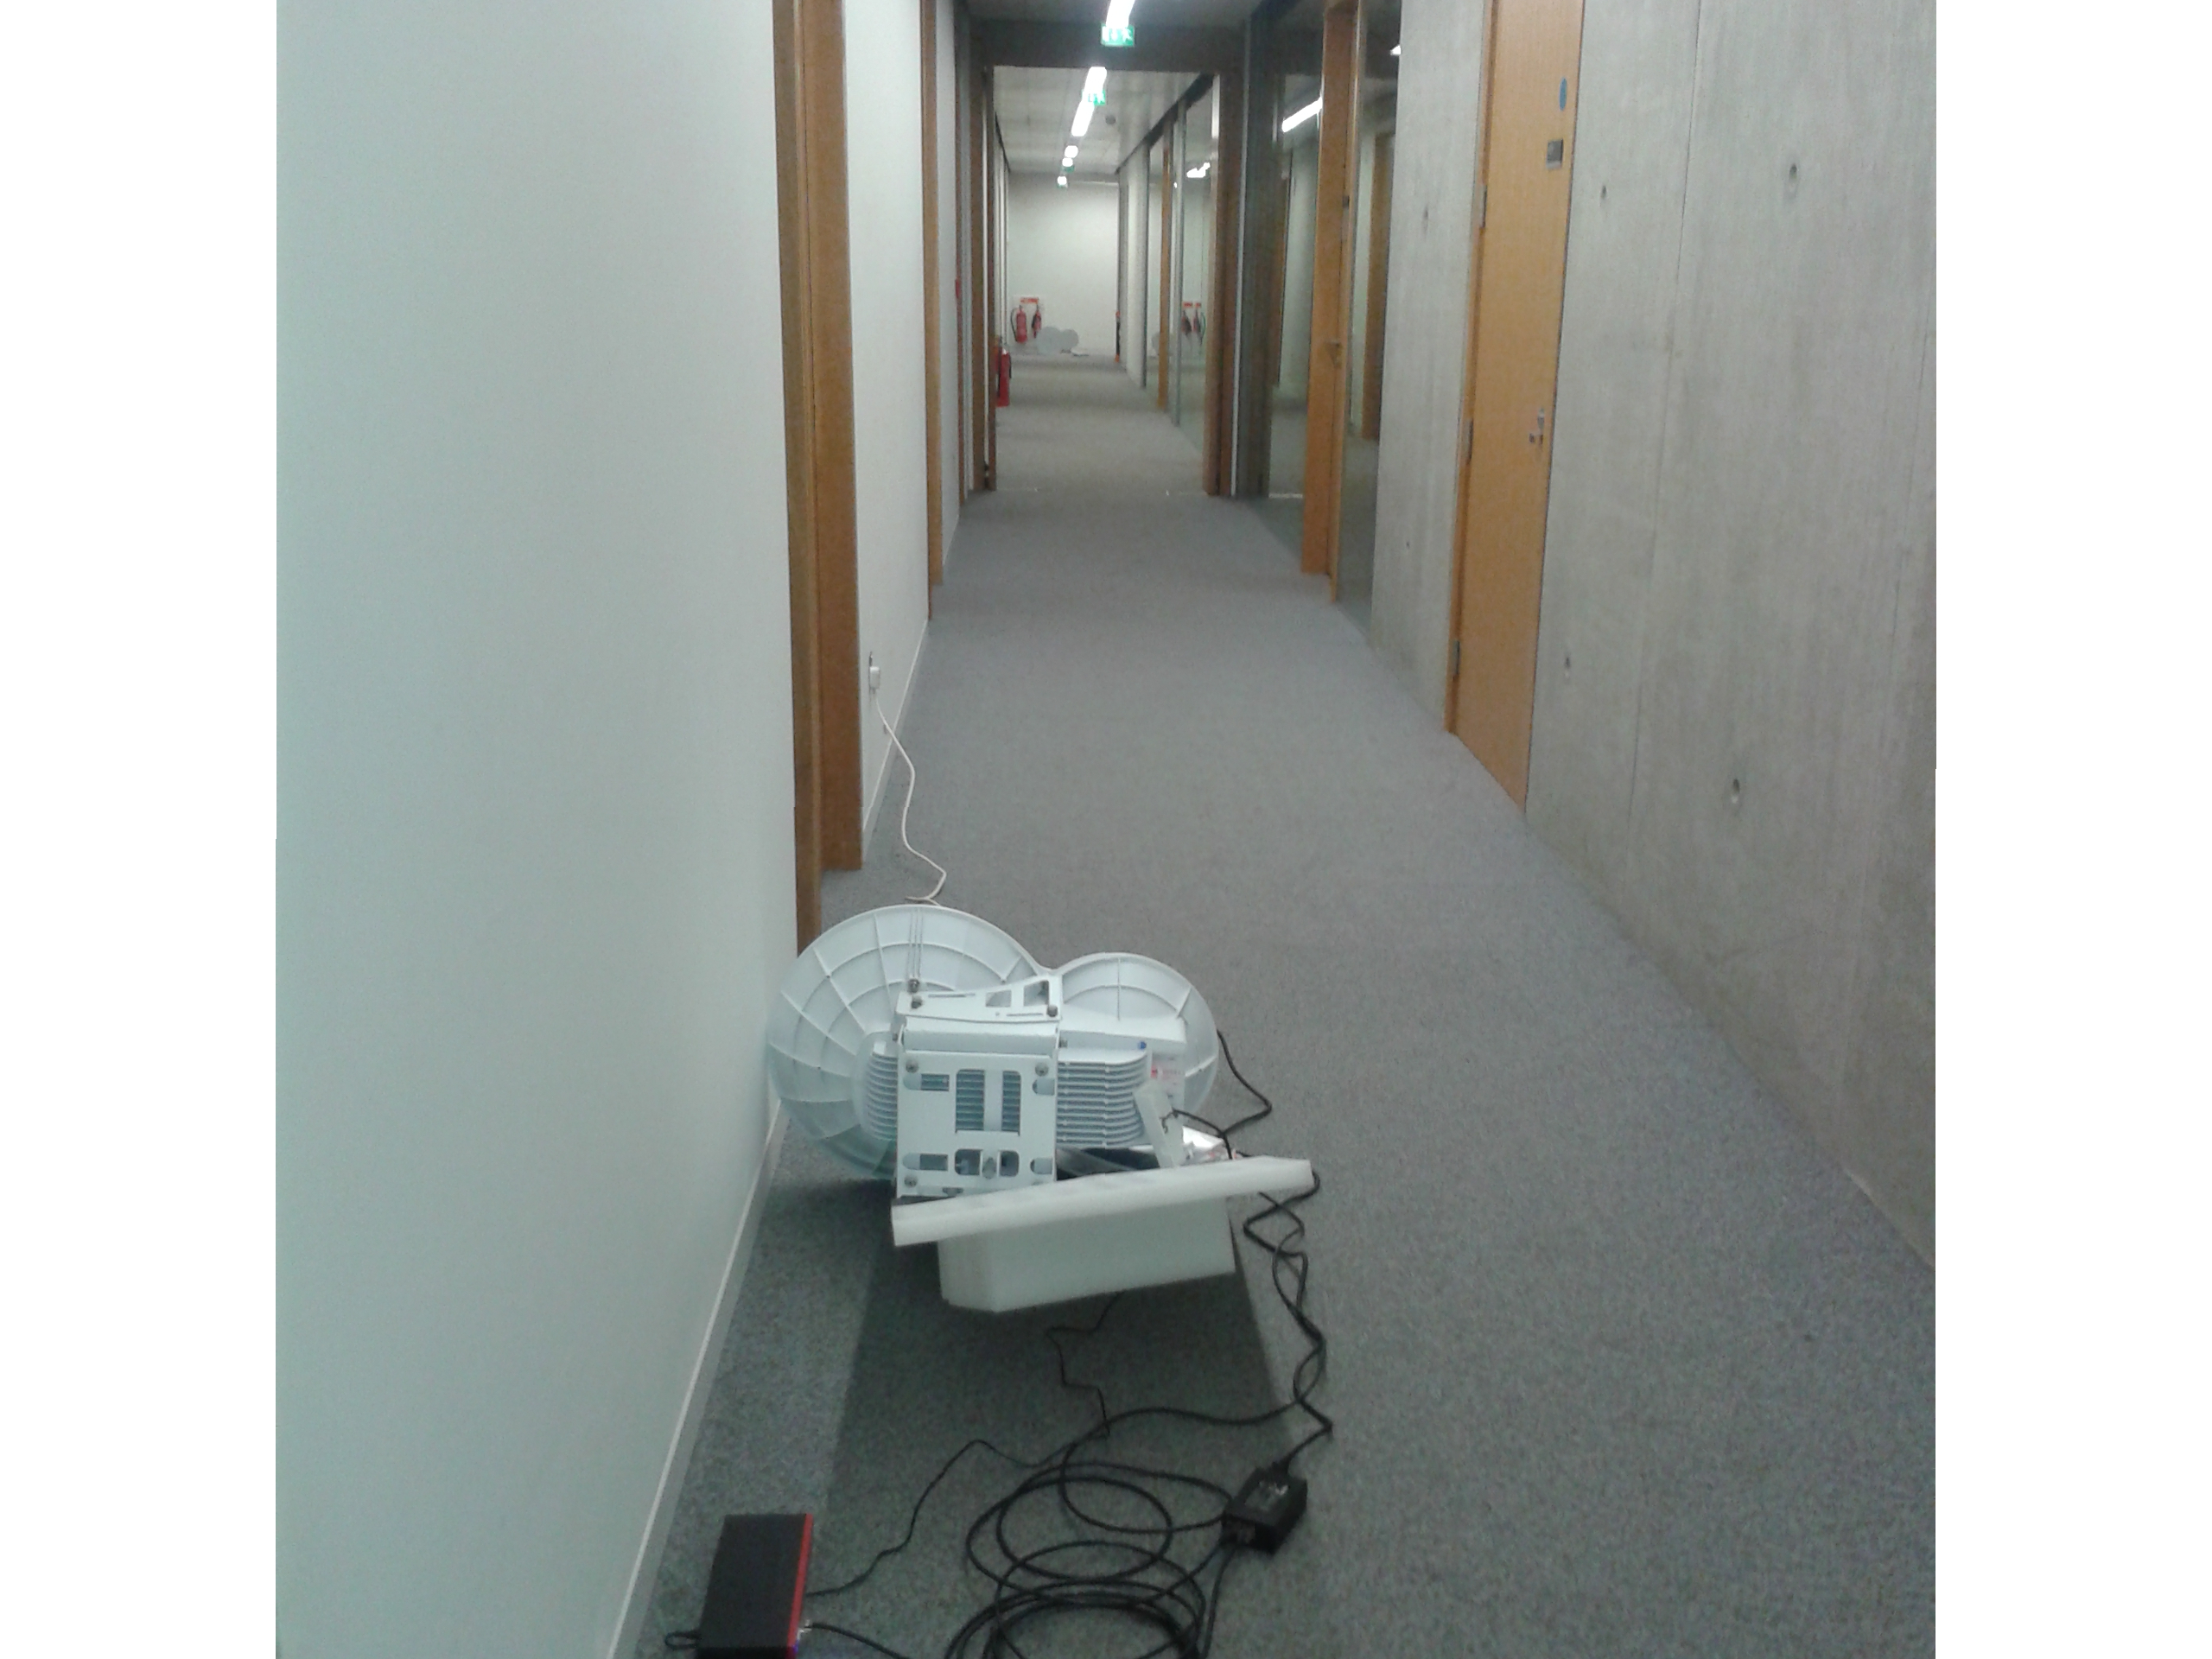
\includegraphics[width=0.3\textwidth]{radio-in-corridor}
\end{wrapfigure}
We ordered and received one pair of radios. Before deploying them
we thought it would be a good idea to check that they were working
and test them in ideal situation -- our office corridor. One thing
we immediately noticed was how critical alignment is. Even over
a distance of 35m, the performance fell of dramatically if the
antennae were slightly out of alignment. It's a very good idea to
configure equipment before deploying it, but to do this we had to turn
off sychronisation which relies on GPS and doesn't work indoors.

\subsection{Strengthening the masts}
\label{december-2013-january-2014-strengthening-the-relays}

Our basic relay construction (see the
\href{http://www.tegola.org.uk/howto/relay-construction.html}{relevant
  howto on the Tegola web site}) uses aluminium pegs to anchor the
diagonal braces to the ground. Both sites were on terrain that
consisted of bedrock covered by peat of varying depth. Although we
have never had a problem with the pegs shifting, peat is a bit
jelly-like, and the structures can wobble through a cm or two. The
alignment of 24GHz is much more critical than for the lower bandwidths
of 2.4 and 5.8GHz, so we replaced the pegs with epoxy bolts into the
bedrock.
\begin{figure}[h]
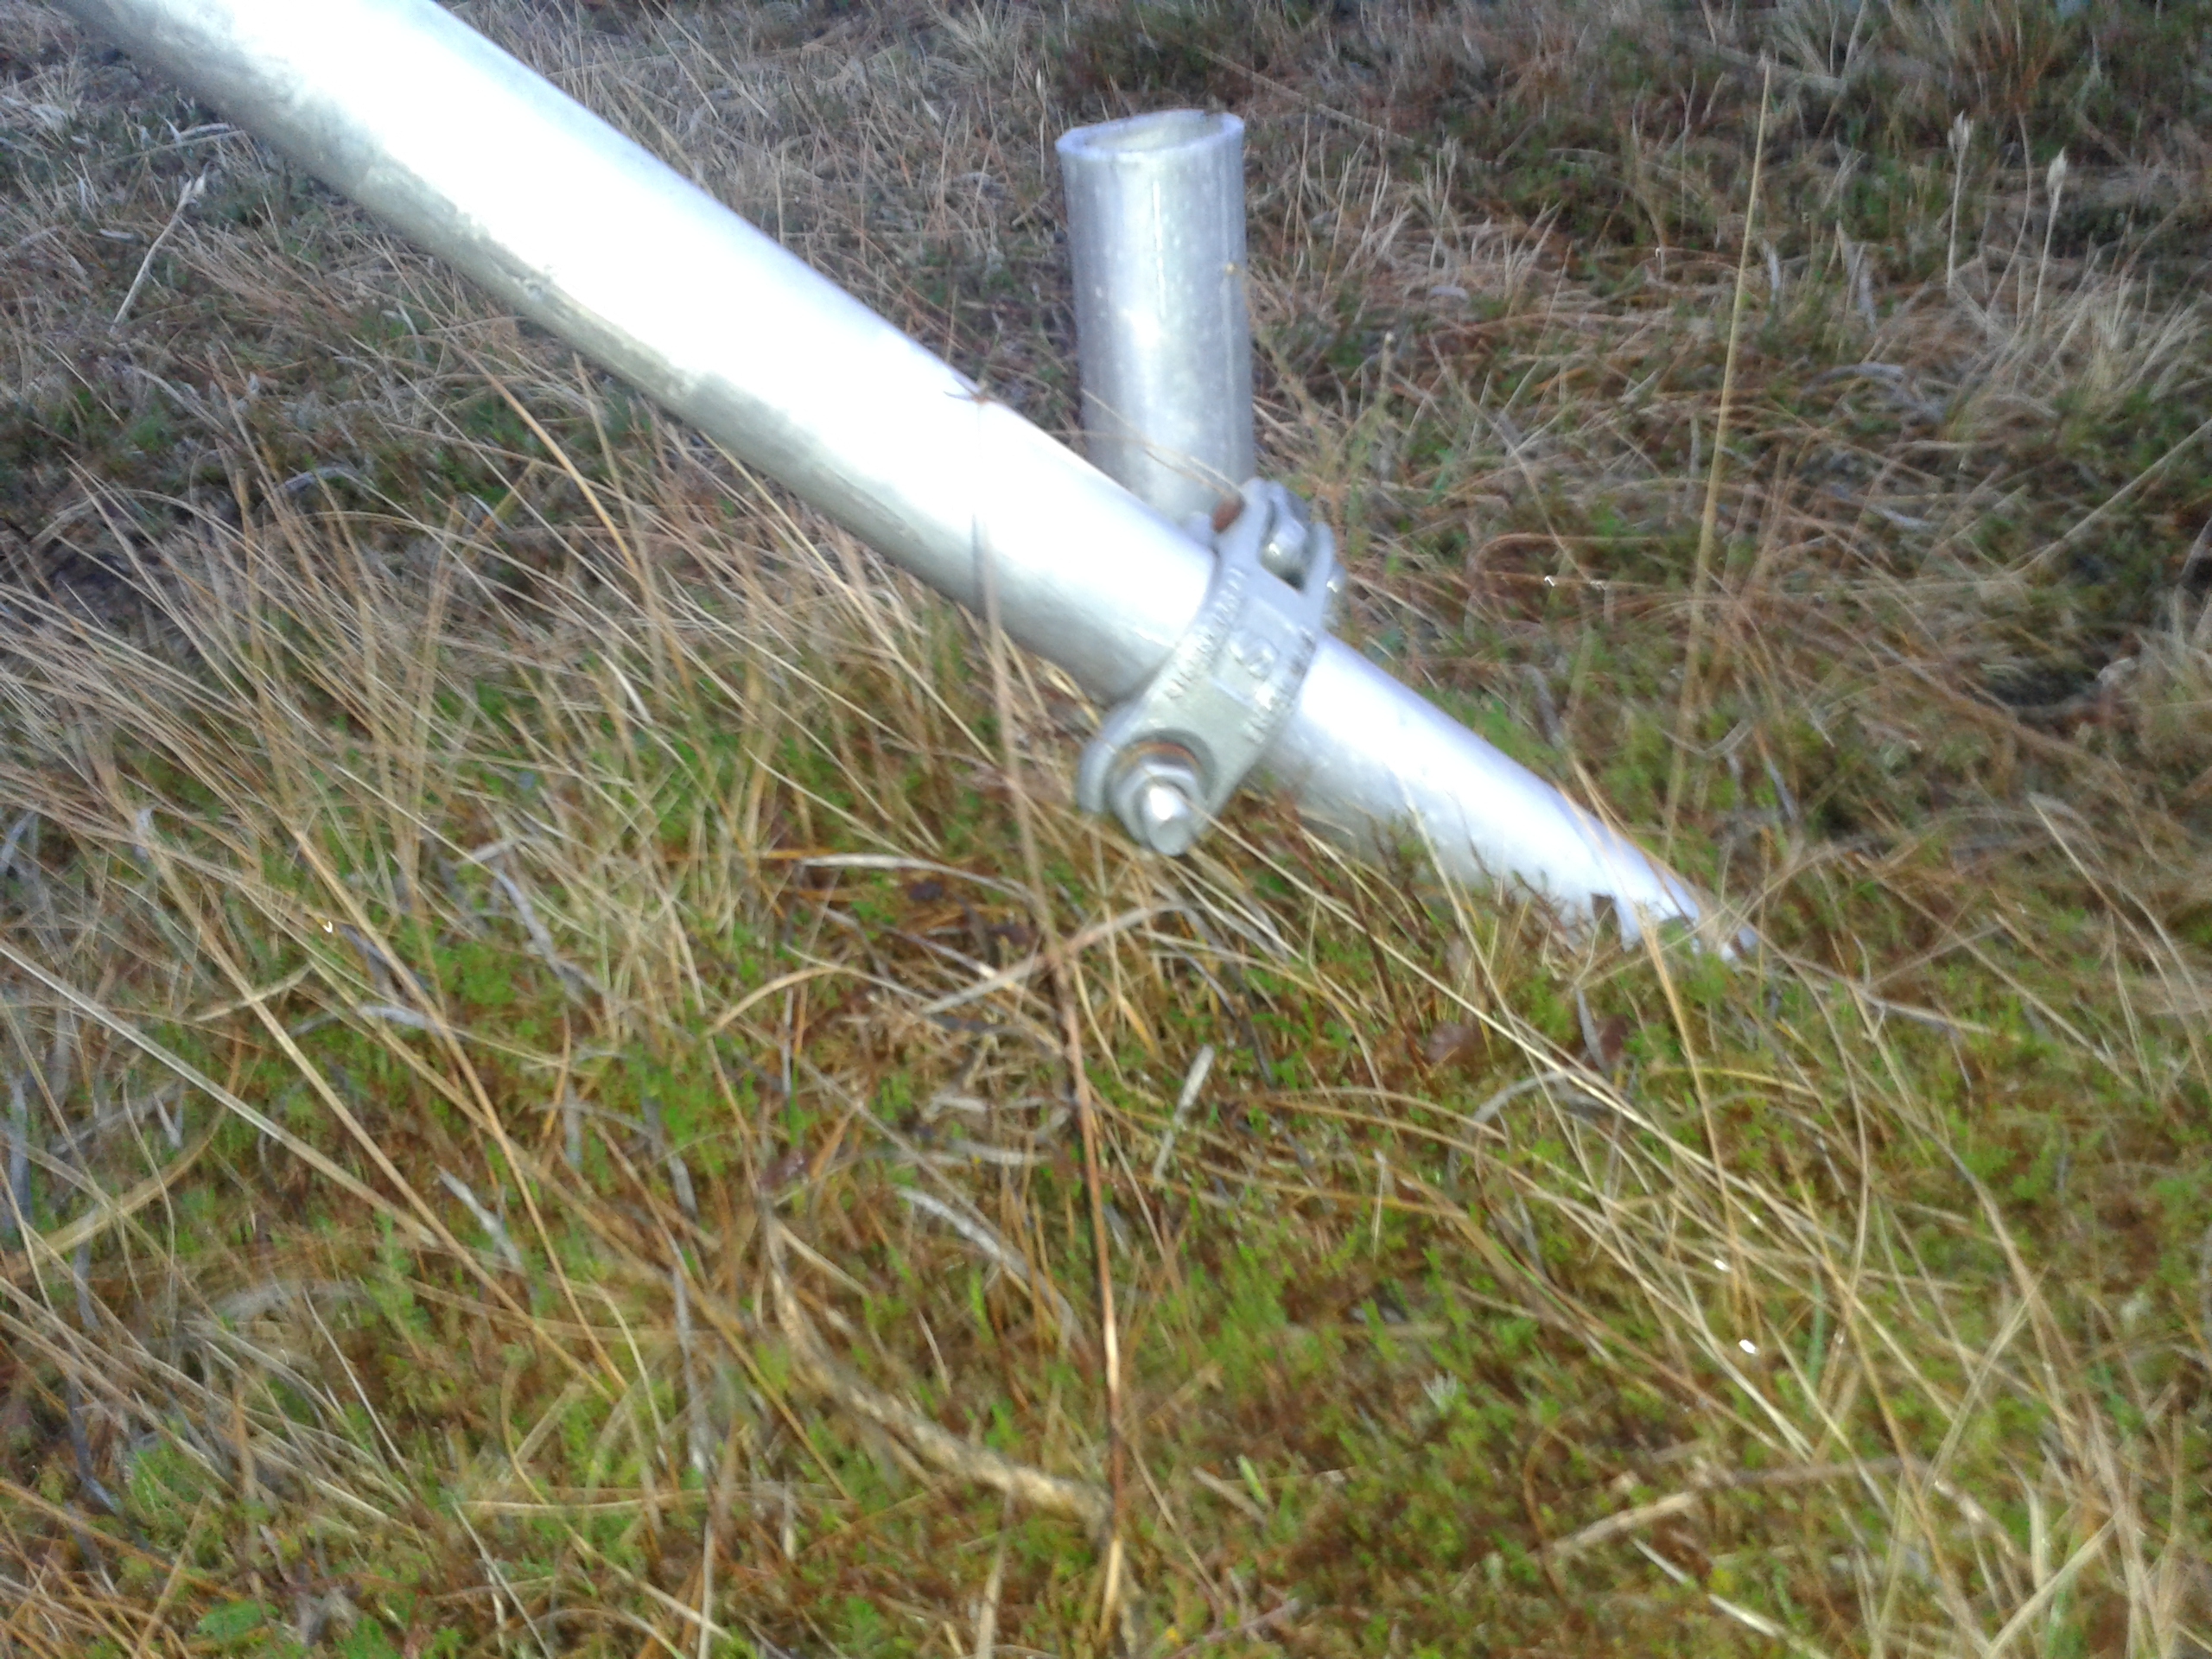
\includegraphics[width=0.4\textwidth]{corran-peg}
\includegraphics[width=0.4\textwidth]{corran-epoxy}
\caption{Pegged anchors (left) and epoxied anchors (right).}
\end{figure}

We also strengthened both relays. For example, at one of our relays we
added an extra horizontal bar.

\begin{figure}[h]
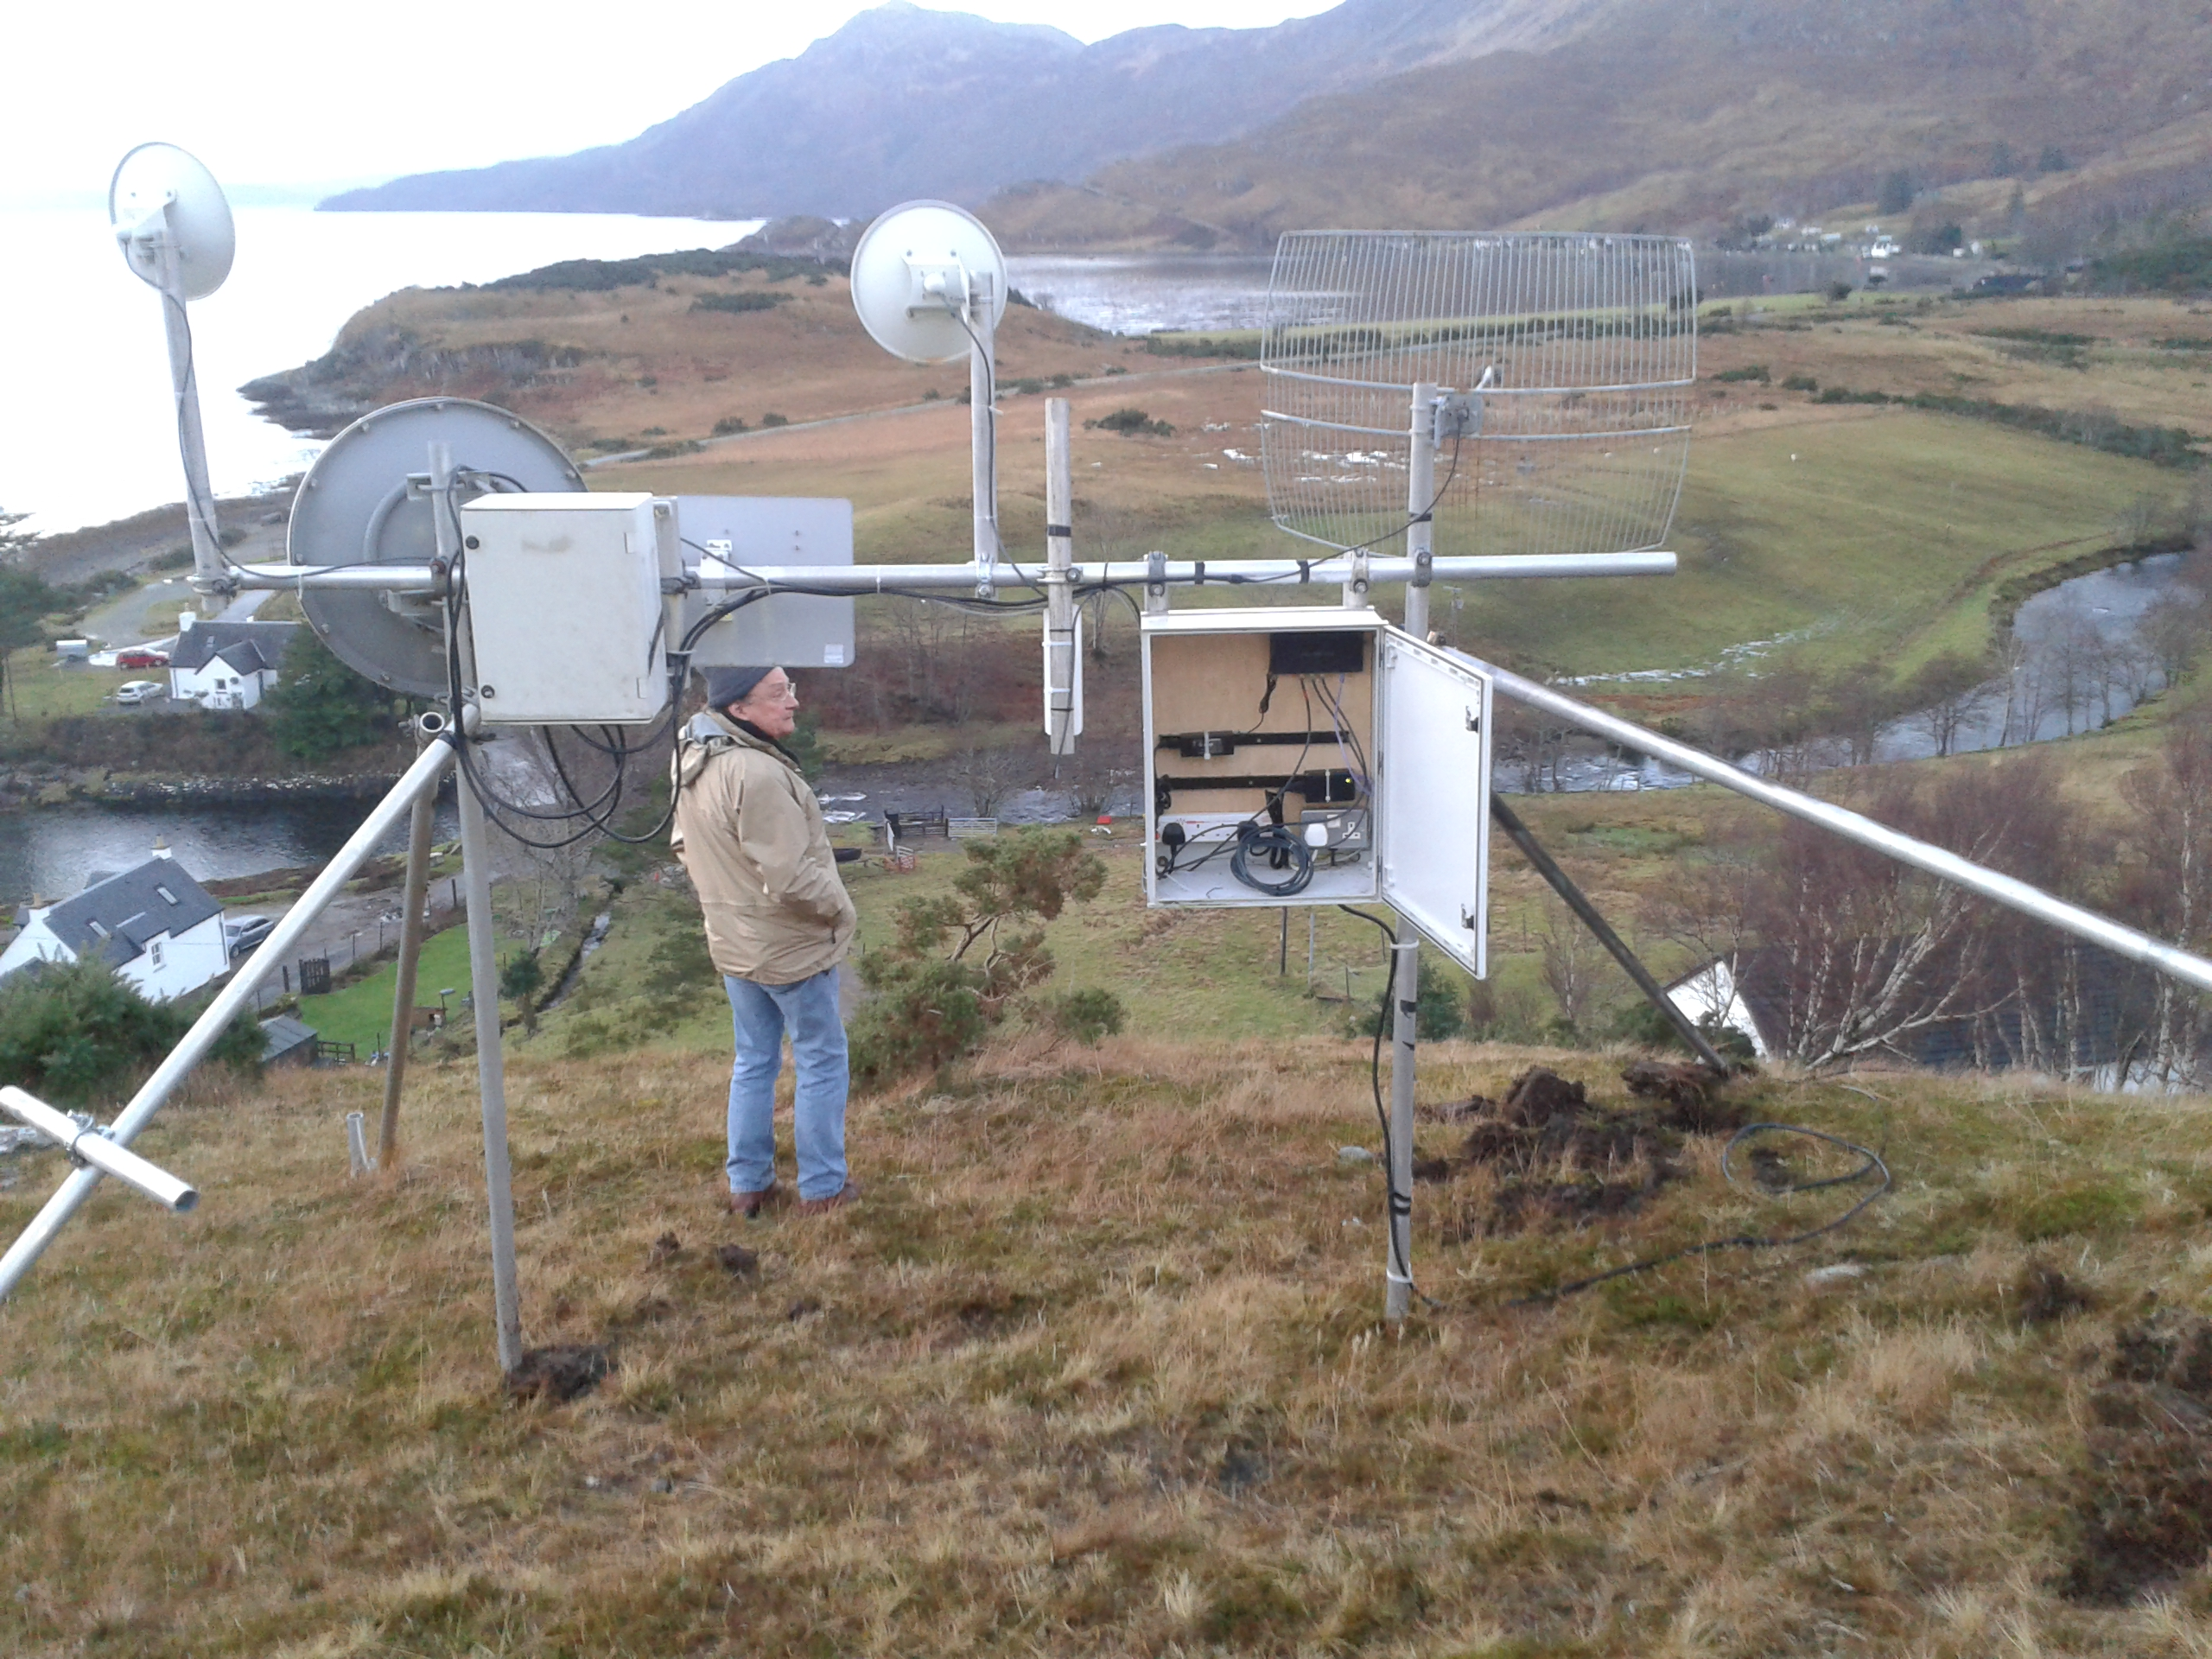
\includegraphics[width=0.4\textwidth]{corran-before-from-behind}
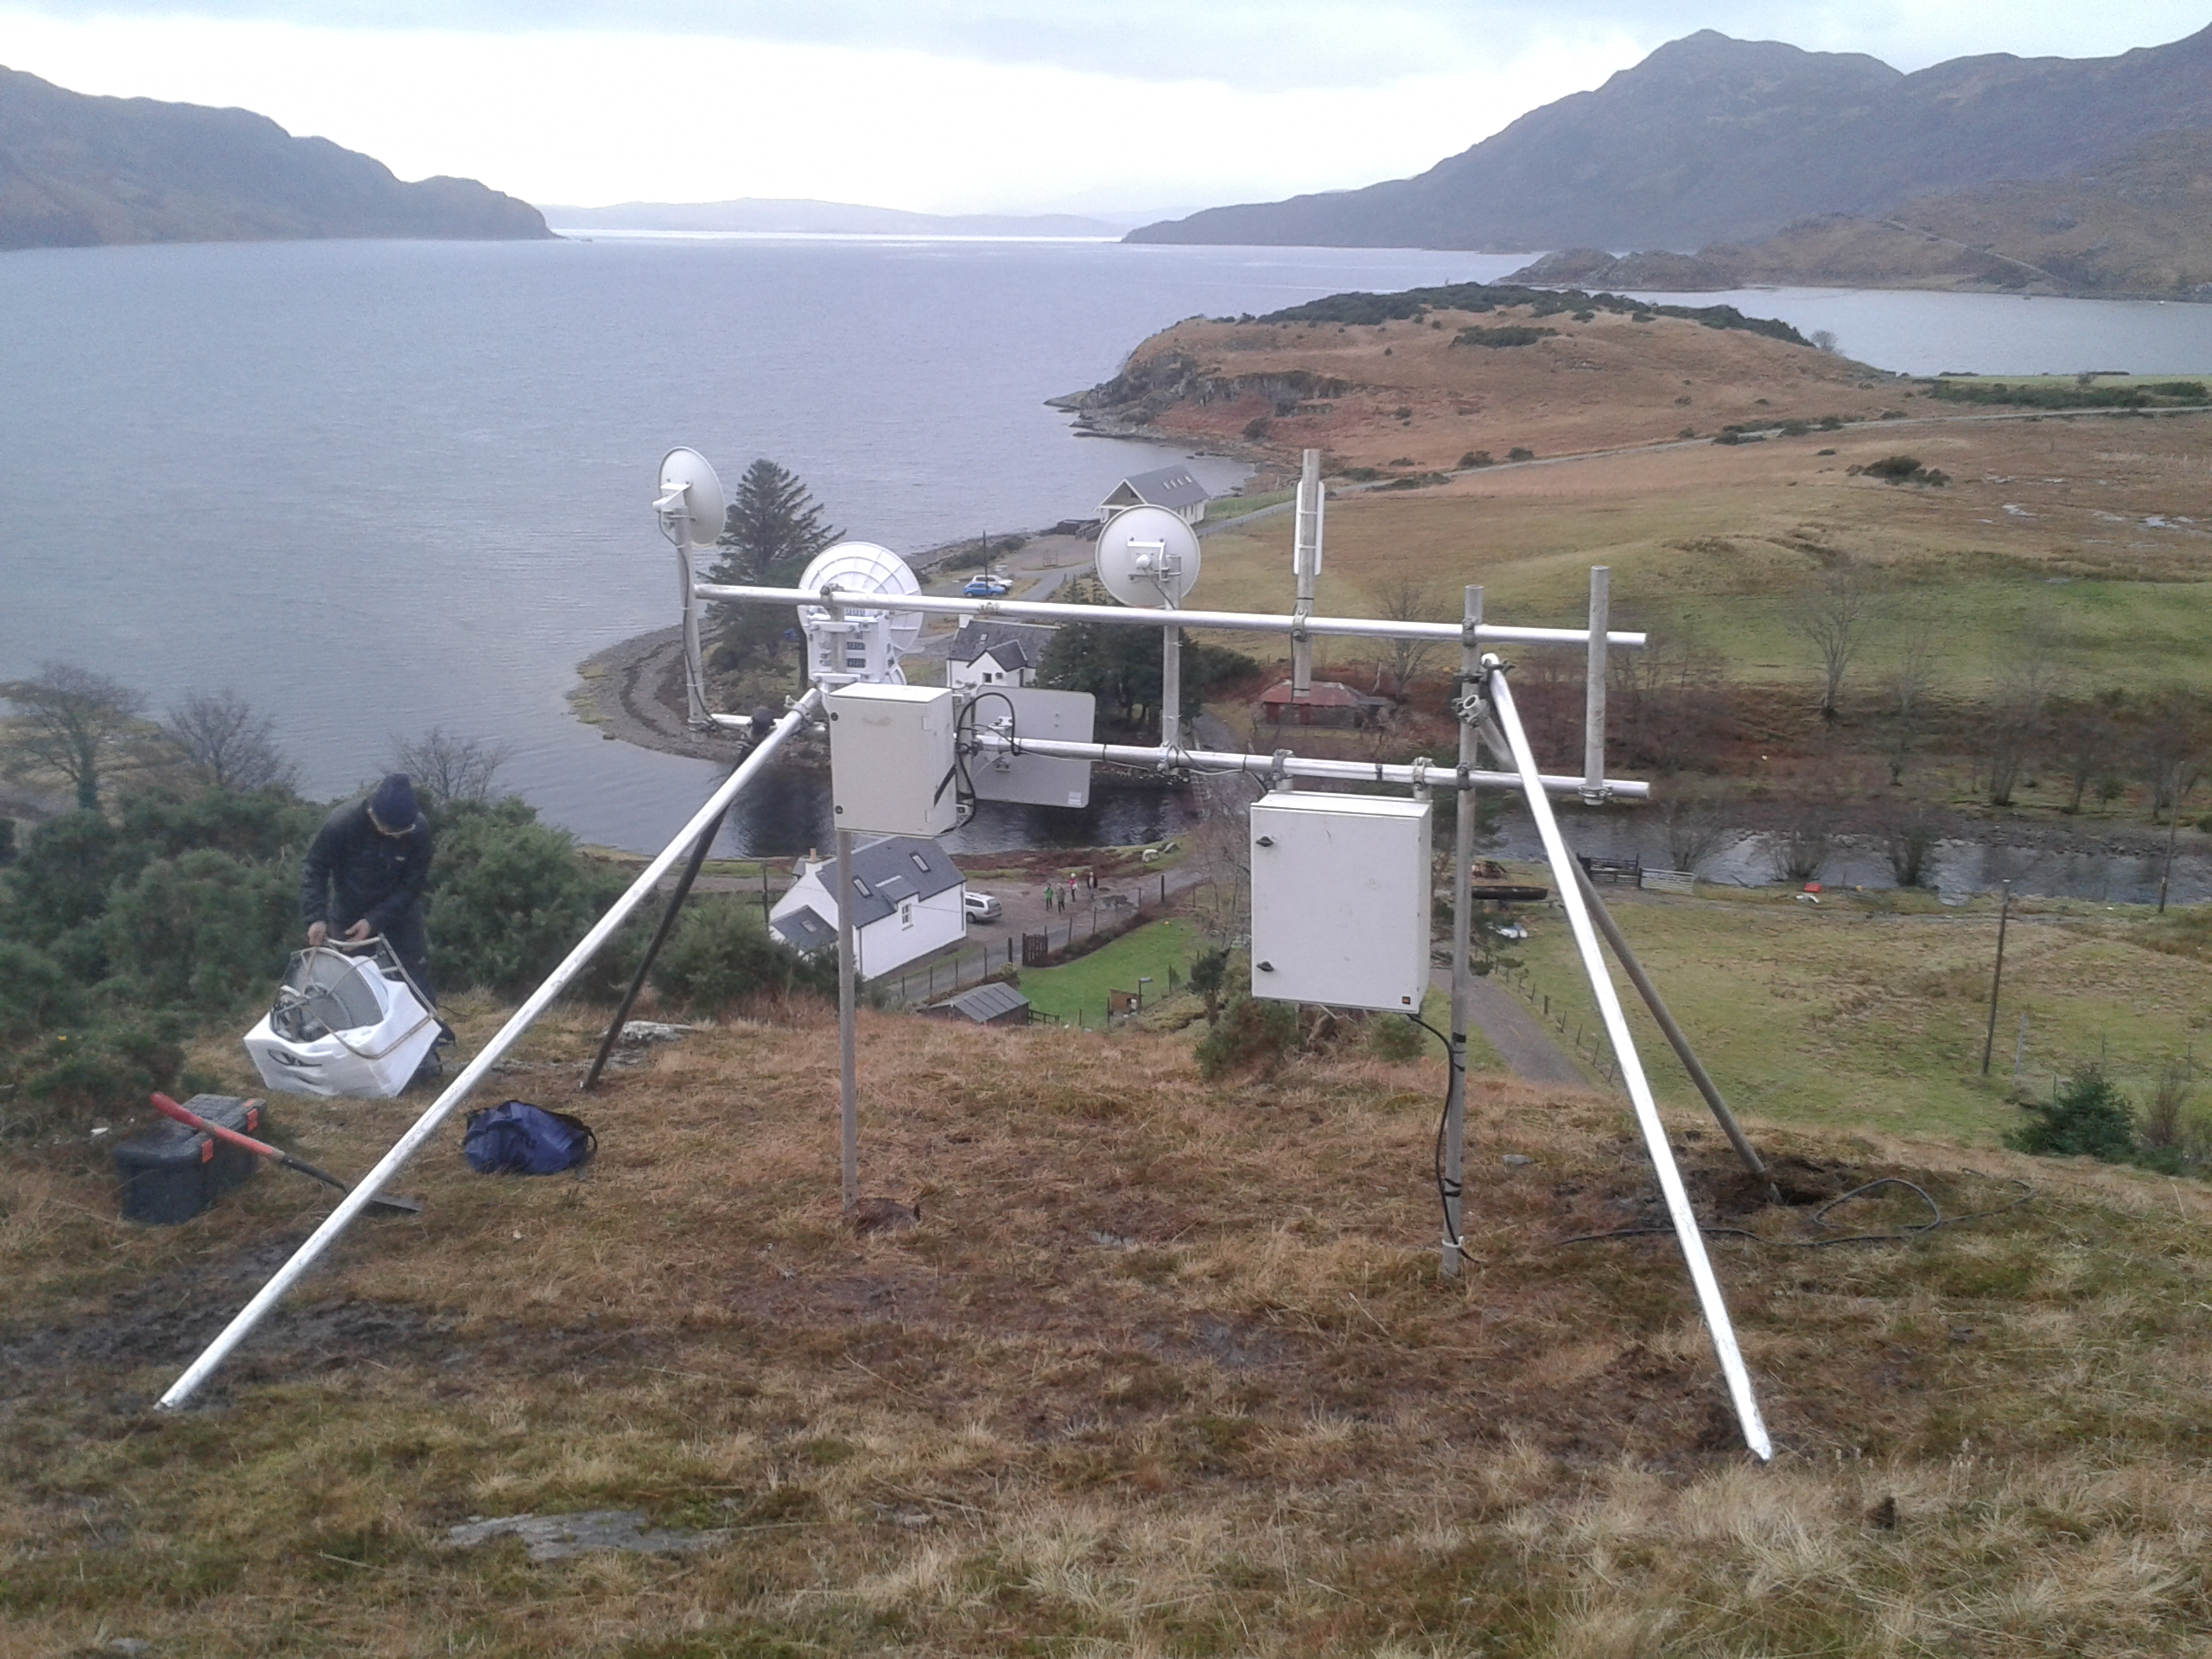
\includegraphics[width=0.4\textwidth]{corran-after-from-behind}
\caption{Corran mast before (left) and after (right)}
\end{figure}

\subsection{Installation and alignment}
\label{january-2014.-installation-and-alignment}

The radios are reasonably light (under 10kg) but awkward to carry up
hills. We used an old backpack frame that 30 years ago had been used
for carrying batteries up to community TV relays. The radios come with
a mounting frame that is first attached to the structure. The radio is
then ``slotted'' into the mounting frame. This arrangement makes it
quite easy to install the whole assembly when working from a ladder.

The antenna can be aligned through elevation and azimuth
adjustment screws. Unfortunately there is a great deal of backlash in
these screws, and they are almost useless if you are working in high
winds. If the clamping bolts are loose, the antenna is blown around
through the considerable travel allowed by the adjustment screws. The
signal strength read-out is at the bottom of the antenna, and if
the alignment is being done from a ladder, you almost certainly
need someone below (with a hard hat) to squint up and call out
the figures.

The installation instructions recommend an alternating process in which
one end of the link is adjusted then the other, and so
on. Unfortunately we were unable to complete this process before
the weather closed in and our workforce departed. However, the
alignment is good enough that we can start taking some measurements.
The initial indications are that the link will work reasonably well
over a distance of 6.5km.

\subsection{Performance}
\label{performance}

\begin{figure}
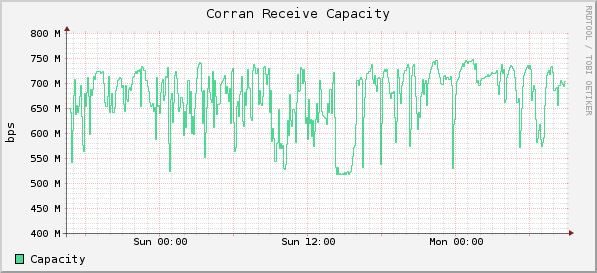
\includegraphics[width=0.6\textwidth]{corran-rcvcap}
\caption{Corran receive capacity...}
\end{figure}
\subsection{Tidal Fading}
Tidal fading has been a serious problem in over water links that 
use to the 2.4 and 5.8 GHz ranges.  They are less of a problem with
higher frequencies (e.g. 24GHz) in which the Fresnel ellipsoids and
beamwidth are narrower~\footnote{our 24GHz link is not over
  water}. The 5GHz Airfiber link operates over a distance of
approximately  20.8km with the two ends at heights of 300m and 20m
above MSL.  We have seen some tidal fading on normal 5GHz transmission
over this link and disruptive fading over the same stretch of water
when both ends are at heights of approximately 20m.

\begin{figure}
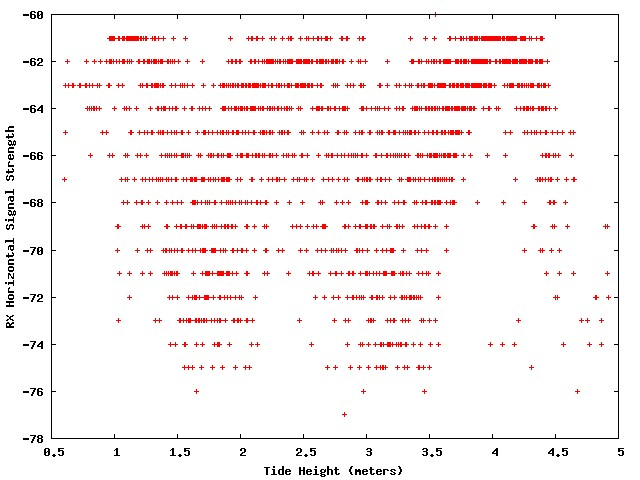
\includegraphics[width=0.7\textwidth]{tidedata/rxpower0.jpg}
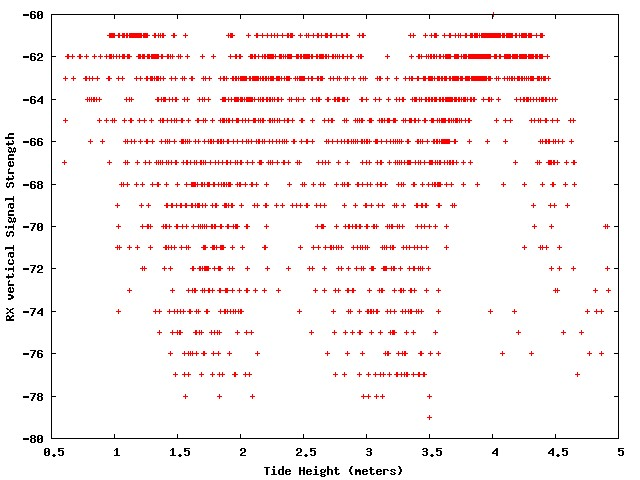
\includegraphics[width=0.7\textwidth]{tidedata/rxpower1.jpg}
\caption{Scatter plot of signal strength against sea level for
  horizontal (top) and vertical  polarizations}
\label{fig:rxpower}
\end{figure}

In January 2015 we had a failure of our the operating link and, since
the weather prohibited climbing up to the 300m high relay, we switched
to the experimental 5GHz Airfiber equipment.
Figure~\label{fig:rxpower} shows the received signal strengths on both
polarizations.  The classic quasi-cycloidal pattern is discernable in
both plots, however it is in a range over with dips to -78 dBm, which
might cause problems.  However these extreme points are probably due
to other causes. Examination of the RX capacity (see
Figure~\ref{capacity} indicates that other effects may dominate tidal
fading and that other things being equal, tidal fading is likely to be
less of a problem on these links than it is on conventional 5GHz
equipment. Readings were taken at 10 minute intervals from mid-January
to mid-February
\begin{figure}
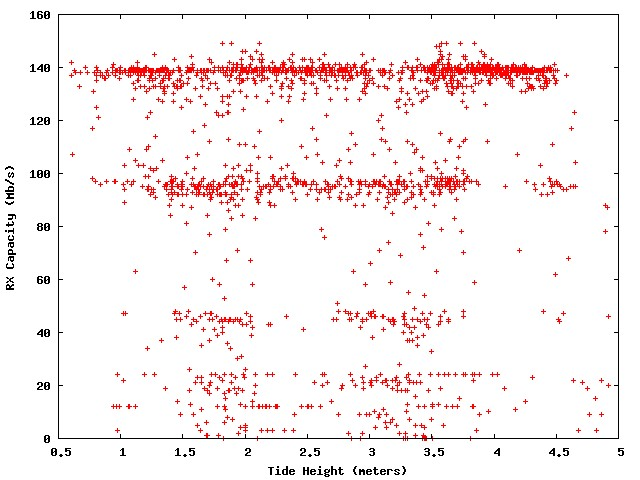
\includegraphics[width=0.7\textwidth]{tidedata/rxcapacity.jpg}
\caption{Scatter plot of signal strength against sea level for
  horizontal (left) and vertical  polarizations}
\label{fig:capacity}
\end{figure}

